% This file was created by matlab2tikz.
%
\definecolor{mycolor1}{rgb}{0.00000,0.44700,0.74100}%
\definecolor{mycolor2}{rgb}{0.85000,0.32500,0.09800}%
%
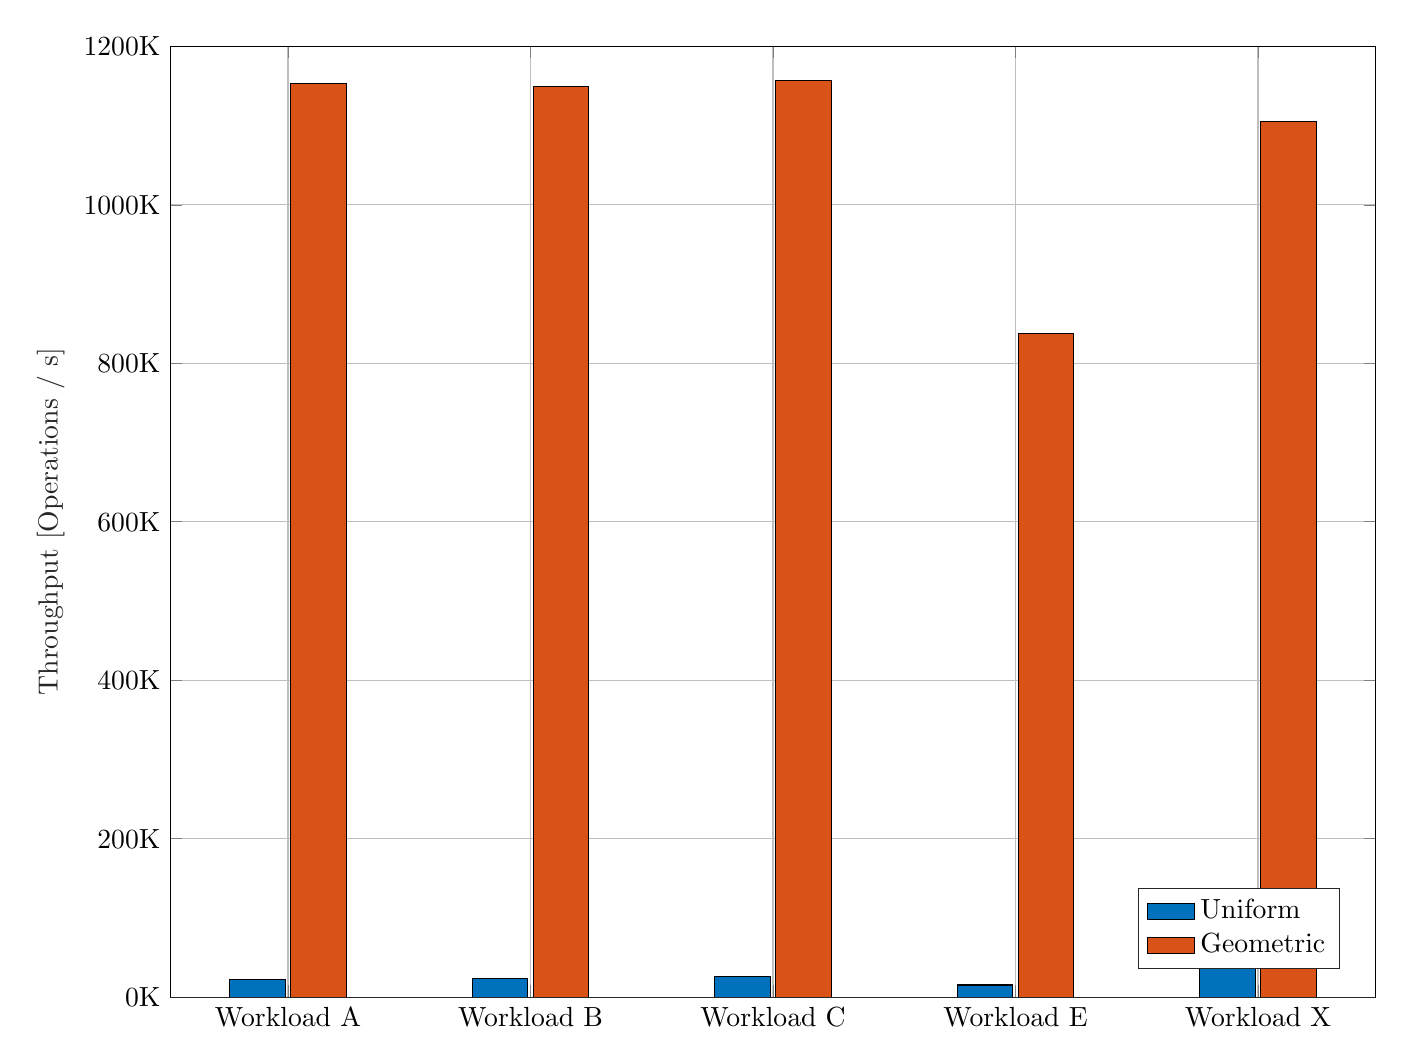
\begin{tikzpicture}

\begin{axis}[%
width=6.028in,
height=4.754in,
at={(1.011in,0.642in)},
scale only axis,
bar shift auto,
xmin=0.514285714285714,
xmax=5.48571428571429,
xtick={1,2,3,4,5},
xticklabels={{Workload A},{Workload B},{Workload C},{Workload E},{Workload X}},
ymin=0,
ymax=1200000,
ytick={0,200000,400000,600000,800000,1000000,1200000},
yticklabels={{0K},{200K},{400K},{600K},{800K},{1000K},{1200K}},
ylabel style={font=\color{white!15!black}},
ylabel={Throughput [Operations / s]},
axis background/.style={fill=white},
xmajorgrids,
ymajorgrids,
legend style={at={(0.97,0.03)}, anchor=south east, legend cell align=left, align=left, draw=white!15!black},
scaled y ticks=false,
scaled x ticks=false
]
\addplot[ybar, bar width=0.229, fill=mycolor1, draw=black, area legend] table[row sep=crcr] {%
1	22813.53\\
2	23814.54\\
3	25644.2\\
4	15310.72\\
5	38669.29\\
};
\addplot[forget plot, color=white!15!black] table[row sep=crcr] {%
0.514285714285714	0\\
5.48571428571429	0\\
};
\addlegendentry{Uniform}

\addplot[ybar, bar width=0.229, fill=mycolor2, draw=black, area legend] table[row sep=crcr] {%
1	1153149.94\\
2	1148874.08\\
3	1156501.77\\
4	837177.97\\
5	1105388.02\\
};
\addplot[forget plot, color=white!15!black] table[row sep=crcr] {%
0.514285714285714	0\\
5.48571428571429	0\\
};
\addlegendentry{Geometric}

\end{axis}
\end{tikzpicture}%